% vim: tw=80

\chapter{Conclusion and Outlook}

In this thesis, triple-differential dijet cross sections were measured forthe
first time using the CMS detector at a center-of-mass energy of \SI{8}{\TeV}.
The constraints on the PDFs of this measurements were studied and the strong
coupling constant \asmz determined.


\begin{figure}[h!tbp]
    \centering
    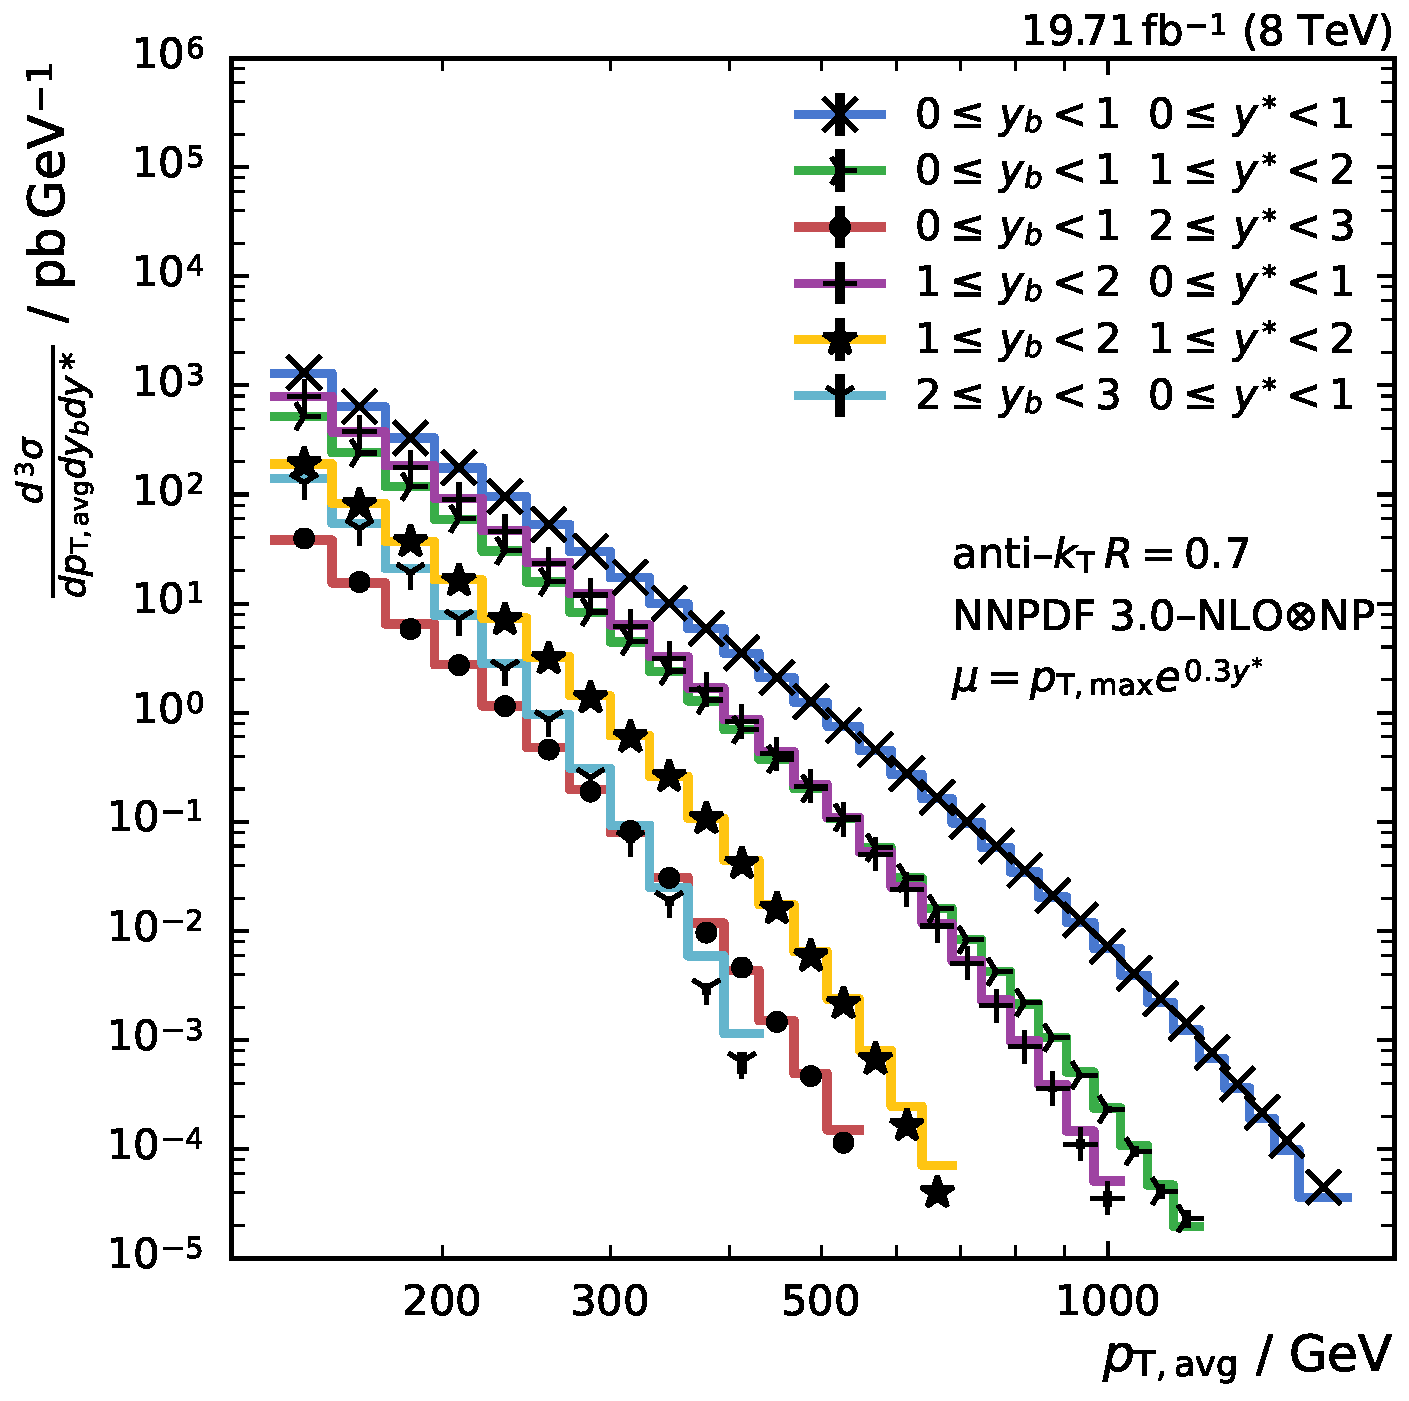
\includegraphics[width=0.4\textwidth]{figures/measurement/ptavg_spectrum.pdf}\hfill
    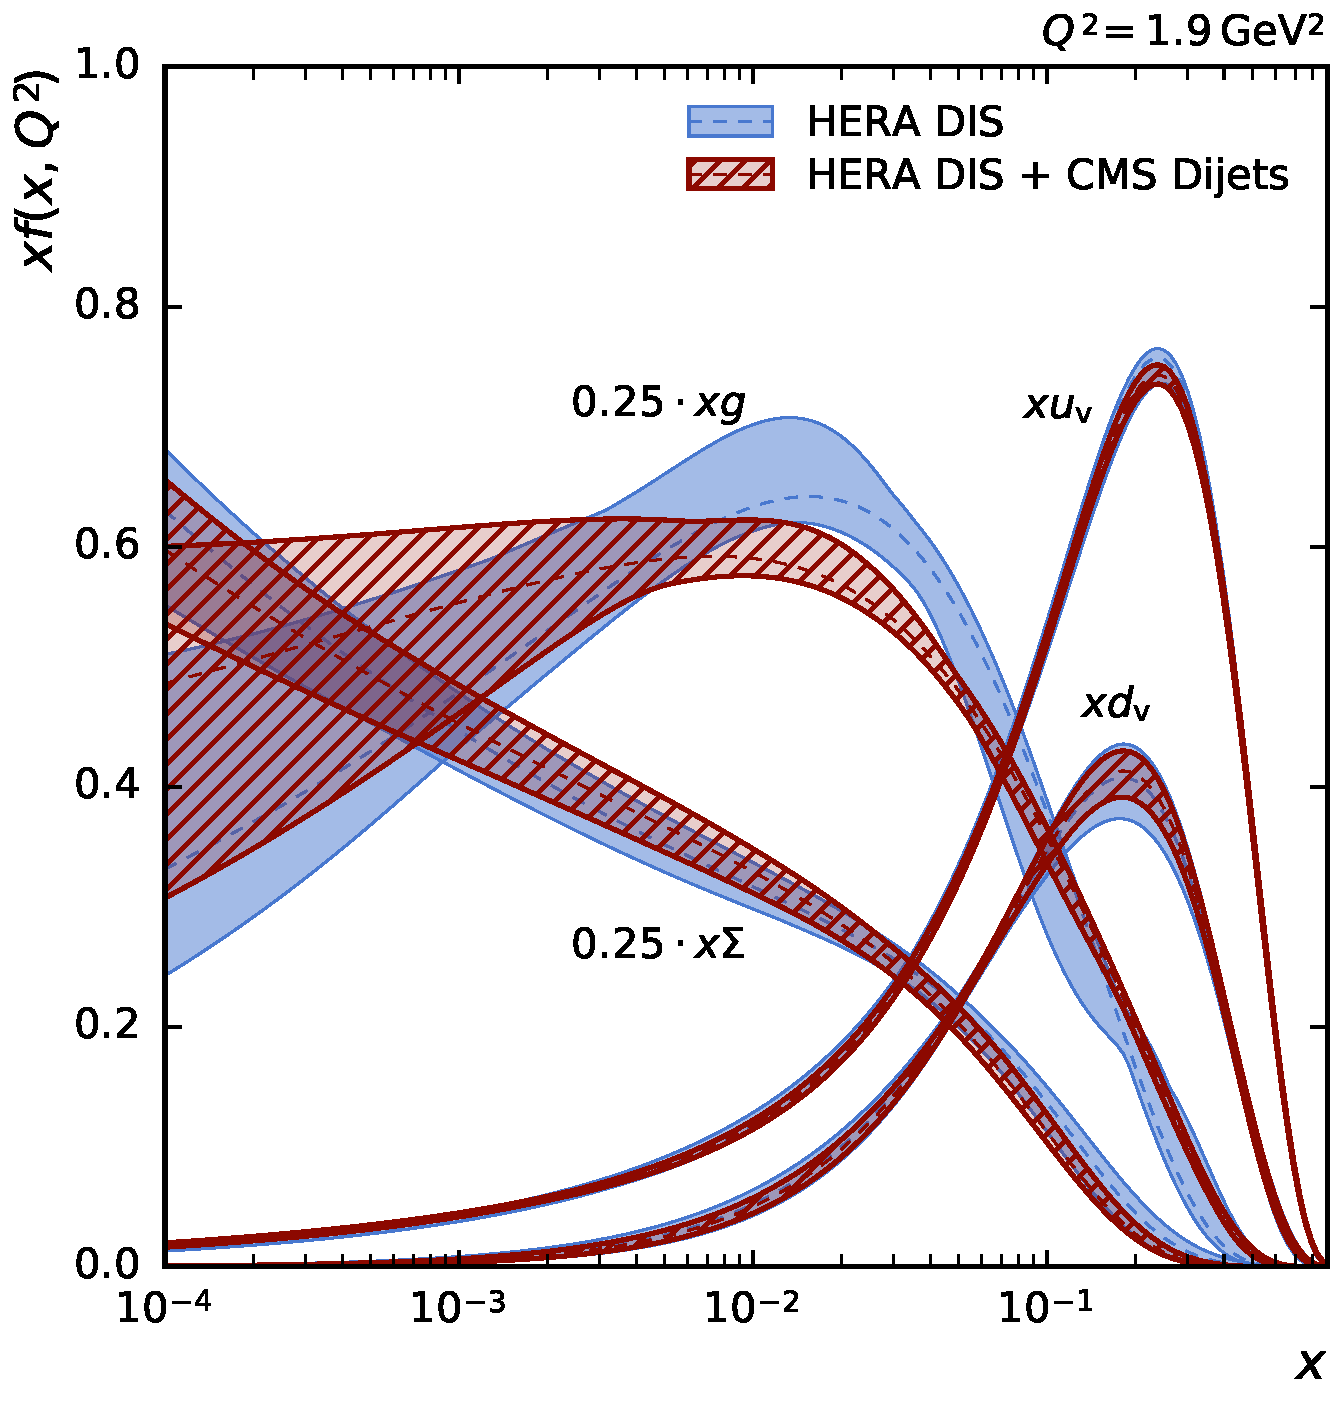
\includegraphics[width=0.4\textwidth]{figures/pdf_constraints/pdfcomp_direct_overview_1.9.pdf}
    \caption[asdf]{asdf}
    \label{fig:conclusion}
\end{figure}
